\begin{frame}
	\frametitle{Herramientas y Tecnologías utilizadas}
	\block{ Android Studio}
		\begin{itemize}
			\item Entorno de desarrollo integrado.
			\item Gradle.
			\item Sistema de depuración sencillo e intuitivo.
		\end{itemize}
	\endblock{}
\end{frame}

%------------------------------------------------------------------

\begin{frame}
	\frametitle{Herramientas y Tecnologías utilizadas}
		\block{\it Node.js}
			\begin{itemize}
				\item {¿Qué es?}.
				\item {¿Por qué se ha decidido utilizar esta tecnología?}.
			\end{itemize}
		\endblock{}
			\begin{center}
				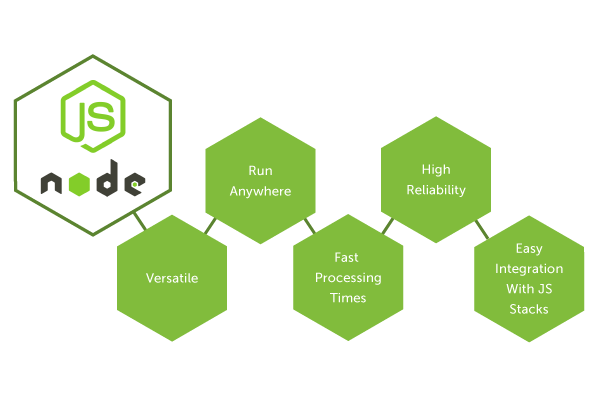
\includegraphics[width=0.72\linewidth]{Images/nodejsfunc}
			\end{center}
\end{frame}

\begin{frame}
	\frametitle{Herramientas y Tecnologías utilizadas}
		\block{\it MongoDB}
			\begin{itemize}
				\item {Base de datos NoSQL}.
				\item {De esquema libre}.
				\item {¿Porqué se ha decidido utilizar MongoDB?}.
			\end{itemize}
		\endblock{}
		\vfill 
		\begin{center}
			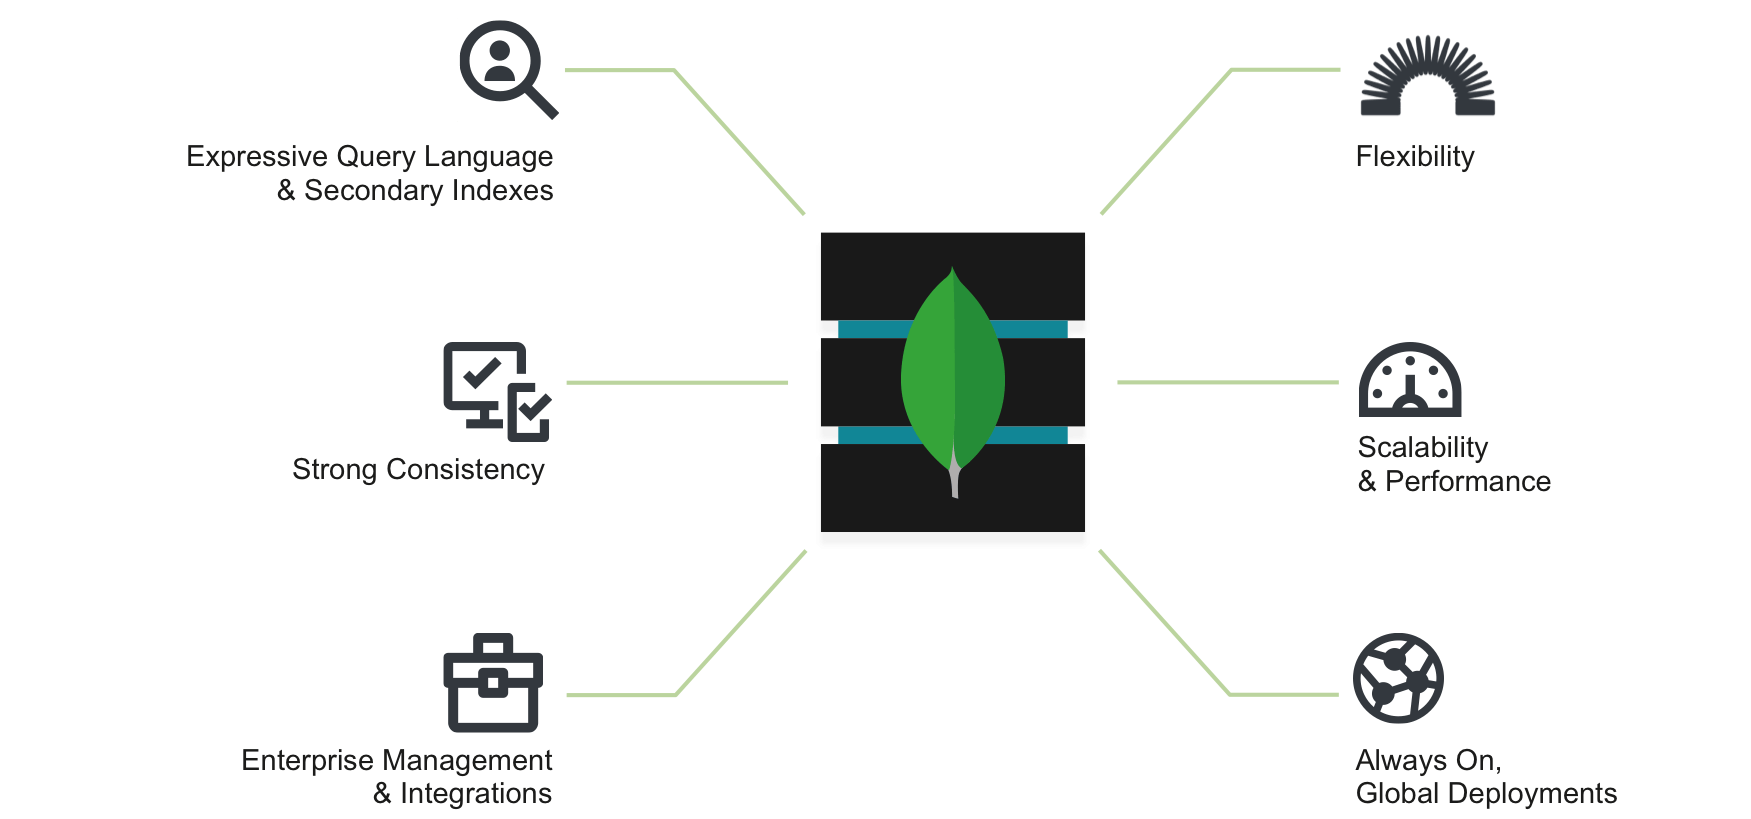
\includegraphics[width=0.88\linewidth]{Images/mongodb-architecture}
		\end{center}
\end{frame}

\begin{frame}
	\frametitle{Herramientas y Tecnologías utilizadas}
	\begin{columns}
			\begin{column}{0.6\textwidth}
				\block{\it Heroku}
					\begin{itemize}
						\item {Plataforma como servicio de computación (PaaS) en la nube}.
						\item {Ejecuta las aplicaciones en ``dynos''.}
						\item {Servidor de \ULLAR{}}.
					\end{itemize}
				\endblock{}
			\end{column}
			\begin{column}{0.4\textwidth}
				\vfill 
					\begin{center}
						
\includegraphics[width=0.9\linewidth]{Images/heroku}
					\end{center}
			\end{column}
	\end{columns}
\end{frame}

\begin{frame}
	\frametitle{Herramientas y Tecnologías utilizadas}
	\begin{columns}
			\begin{column}{0.6\textwidth}
				\block{\it mLab}
					\begin{itemize}
						\item {Servicio de base de datos en la nube.}
						\item {Ofrece bases de datos MongoDB}.
						\item {Ejecuta sus máquinas en proveedores de servicios en la nube como AWS, Azure y Google Cloud.}
						\item {Base de datos de \ULLAR{}.}
					\end{itemize}
				\endblock{}
			\end{column}
			\begin{column}{0.4\textwidth}
				\vfill 
					\begin{center}
						
\includegraphics[width=0.8\linewidth]{Images/mlab}
					\end{center}
			\end{column}
	\end{columns}
\end{frame}

\begin{frame}
	\frametitle{Herramientas y Tecnologías utilizadas}
		\block{\it Google Maps}
			\begin{itemize}
				\item {API de Google Maps.}
				\item {Permite integrar los mapas de Google Maps en una aplicación Android.}
				\item {Permite:}
				\begin{itemize}
					\item {Creación de marcadores, polígonos y superposiciones.}
					\item {Cambiar la vista del mapa.}
					\item {La posibilidad de elegir el tipo de mapa}
				\end{itemize}
			\end{itemize}
		\endblock{}
\end{frame}

%--------------------------------------------------------------------
